\begin{document}
We are going to touch on some essential features and metrics that characterize a network.

\section{Sharing}
Sharing is an essential part of networks, as we can reduce the amount of long links needed to connect multiple devices. 
\begin{figure}[!htbp]
    \centering
    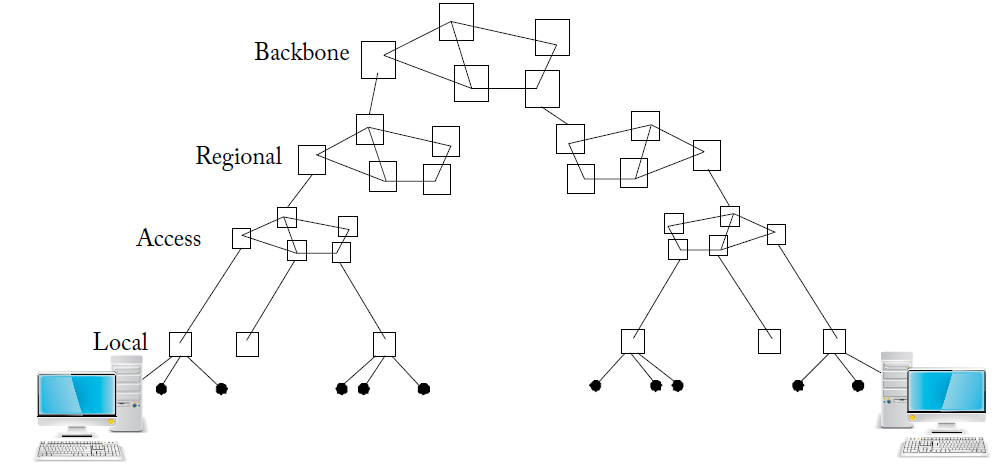
\includegraphics[width=0.75\textwidth]{fig2_1_networkhierarchy}
    \caption{Hierarchy of networks where multiple devices are sharing a local network, multiple local networks are sharing an access networks, and so on}
    \label{fig:Network_Hierarchy}
\end{figure}
\subsubsection*{Multiplexing Gain}
Sharing is possible because devices are not active all of the time. Multiplexing gain measures the benefit of sharing a link between many users and is the amount of active users sharing a link. If $C$ is the link data rate, $M$ is the multiplexing gain, and $C_{user}$ is the data rate seen by the user.
$$ C_{user} = C/M $$
ex. A thousand users are sharing a link, but only ten are active.
$$ C_{user} = C/10 bps$$

\section{Link Metrics}
\subsubsection*{Link Rate}
Each link is characterized by data rates in bits per second.
ex. Common link rates for cable modem uplink (device to Internet) are 131 Mbps and downlink rate (Internet to device) are 343 Mbps. \\
ex. Links are broadband if its rate exceeds 25 Mbps
downlink and 4 Mbps uplink. If its rate does not exceed that amount it is considered narrowband.
\subsubsection*{Frequency}
Cycles per second (Hz). \\
ex. $V(t) = A sin(2 \pi f_0 t)$, $f_0$ is the frequency
\subsubsection*{Bandwidth}
Measures the width of the range of frequencies on a link.\\
ex. A telephone line can transmit signals over a range of 300 Hz to 1 MHz, so the bandwidth is $$10^6 - 300 = 999700 Hz \approx 1 Mhz$$
\subsubsection*{Signal to Noise Ration (SNR)}
The ratio of the power of the signal at the receiver over the power of the noise at the receiver. Sometimes given in dB, but we would link the ratio. 
$$dB = 10log_{10}(ratio)$$
\subsubsection*{Shannon Capacity}
The larger the bandwidth of a link the faster the link rate. The noisier the channel is, the smaller the SNR, and the more bandwidth needed to reliably transmit the signal. Shannon Capacity quantifies the relationship between the $C$ the maximum reliable link rate, $SNR$ the noise, and $W$ the bandwidth. It is also the theoretical link rate limit that can be achieved. 
 $$C = Wlog_2(1+SNR)$$

\section{End to End Metrics}
\subsubsection*{Delay}
The elapsed time for a packet to traverse between two points. Queuing time is the waiting time for a packet at a node before it can be transmitted. Transmission time refers to the time it takes for a packet to be transmitted over a link at the link rate. Propagation time is the time for the physical signal to get from the starting point to the ending point. Processing time is the time consumed to performing the required operations to process a packet at a node. 
$$Delay_{A\_to\_B} = Q/R + P/R + T_{propagation}$$
$$Delay_{A\_to\_C} = Q/R + 2P/R + T_{processes} + 2T_{propagation}$$

\begin{figure}[!htbp]
    \centering
    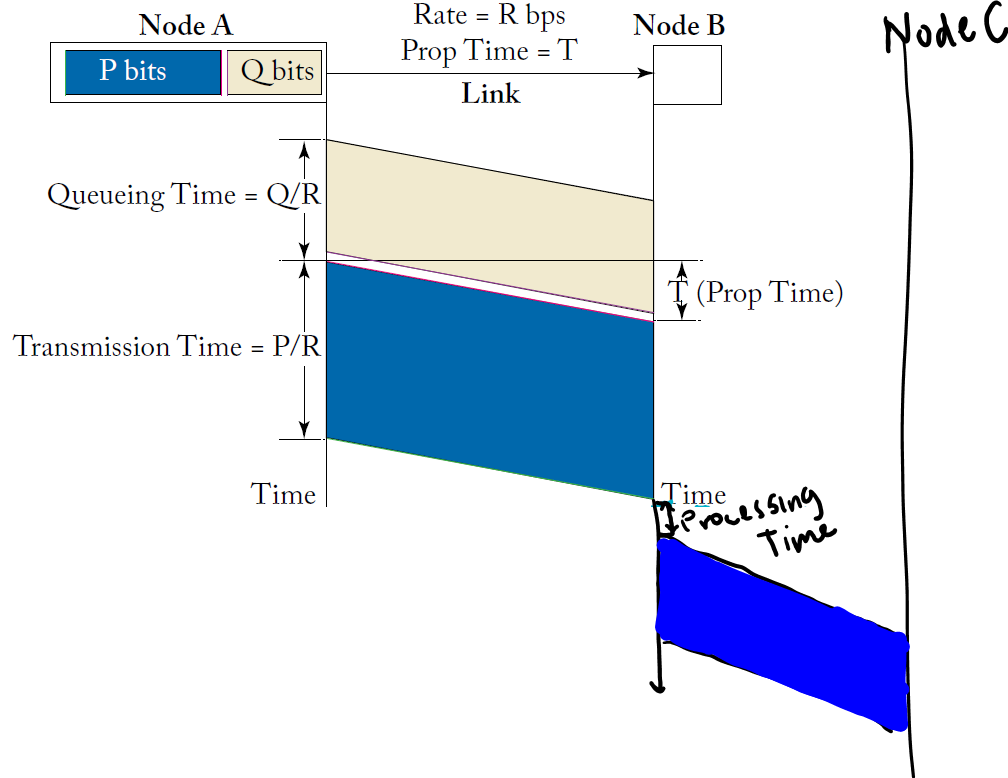
\includegraphics[width=0.5\textwidth]{fig2_2_delay}
    \caption{Delay from Node A to Node B to Node C}
    \label{fig:Delay}
\end{figure}

\subsubsection*{Outstanding Packet}
Status of a packet is outstanding if the sender has transmitted the packet but has not received an acknowledgement.
\subsubsection*{Window Size}
The maximum allowed number of outstanding bytes.
\subsubsection*{Round-Trip Time}
The time between sending out a packet and recieving an ack.
\subsubsection*{Throughput}
Data rate for a particular application, bits per second. Not the same as link rate, because particular applications may send a sequence of packets with gaps between each of the packet transmissions. \\
ex. A source $S$ sending a packet to a destination $D$. Lets say there is a window size of three packets, so the sender can only sent three packets betfor waiting for an acknowledgement. The throughput of this application is less than the link rate, because of the time that the sender has to wair for an acknowledgement. 
\begin{figure}[!htbp]
    \centering
    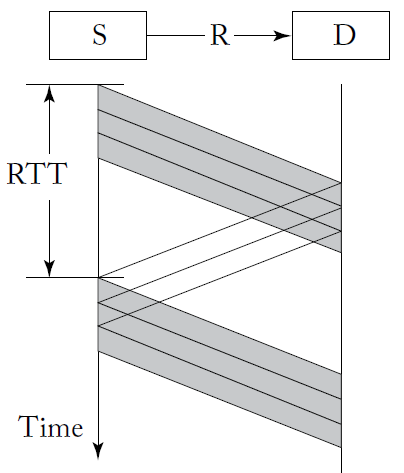
\includegraphics[width=0.5\textwidth]{fig2_3_tp_window}
    \caption{Throughput limited by window size}
    \label{fig:tp_window}
\end{figure}
\\ ex. If multiple devices $A$, $C$, and $D$ are linked to a router $B$. If $A$ wants to send information to $C$ and $D$, the throughput of the connection from $A$ to $C$ is $R/2$ and from $A$ to $D$ is $R/2$, because the maximum rate from $A$ to $B$ is only $R$. 
\begin{figure}[!htbp]
    \centering
    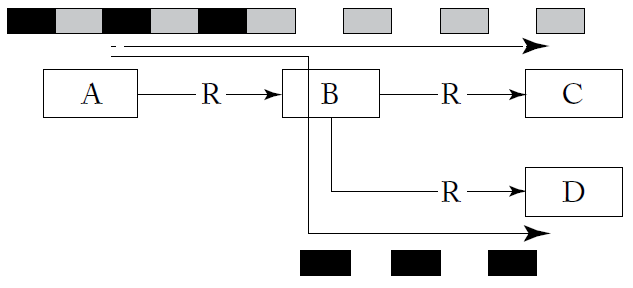
\includegraphics[width=0.5\textwidth]{fig2_3_tp_bottleneck}
    \caption{Throughput limited by bottleneck link}
    \label{fig:tp_bottleneck}
\end{figure}

\subsubsection*{Delay Jitter}
The difference between the longest and shorted delivery time among the packets of that connection. Successive packets sent may not face the same delay accross a network due to congestion or other issues. \\
ex. For streaming applications, a constant stream of packets in necessary. Lets say that the delay jitter $J$ is known. The destination can store the packets that arrive in a buffer. Then, the first packet should be stored for $J$ seconds before playing it back, and the subsequent packets should be able to be streamed from the buffer.
\subsubsection*{M/M/1 Queue}
Memoryless arrival, Memoryless service, 1 server model that allows us to estimate the delay and backlog at transmission lines. Let us discretize our example into 1 second intervals and assume that the probability a packet arrives each second is $\lambda$ and the probability the server finishes servicing a packet each second is $\mu$. \\
Average service time per packet is $\frac{1}{\mu}$ \\
Utilization of the system is $\rho = \frac{\lambda}{\mu}$ \\
Average time that a packet spends in a buffer or being served$T = \frac{1}{\mu-\lambda}$ \\ 
Average queueing time $T-\frac{1}{\mu}$\\
Average number of packets  stored in a link's transmitter queue $L = \frac{\lambda}{\mu}$



\end{document}